\documentclass[12pt]{article}
\usepackage{amsmath, amssymb, amsthm, graphicx, epsfig, fancyhdr, graphicx, amsfonts}
\usepackage{algorithm}
\usepackage[noend]{algpseudocode}
\usepackage[utf8]{inputenc}

\title{Math 240 Overleaf Form} 
\author {Laouen belloli}

\setlength{\headheight}{28pt}
\pagestyle{fancy}
\fancyhf{}
\fancyhead[R]{Laouen Belloli \\ Automatic creation of Metabolic Network in PDEVS}
\fancyfoot[C]{\thepage}


\begin{document}

\section*{summary of the reading}
After spend 3 days reading both books,''Principles of Biochimistry`` from Lehninger and ''Chemistry \& Chemical Reactions``  from Kotz \& Treichel, I restart with another diferent aprouch to the problem.

Since we only want to consider reaction leaded by enzymes, I don't see why to model the reactions instead of model the cell components. A cell have many components and fenomens, but we can only model these components and fenomens needed. In this way, in the future, we can add others components or fenomens as we'll need it.


\section*{new aprouch for the cell model}  
A cell have basicly three components that matter for us, a membrane (where transportation reactions happens), a cytoplasm (where some reaction happens) and organelles (different compartments with their own reactions).
There is a lot of other components but I am not considering them.
all this components have enzymes and therefore reaction happens there. the membrane is who take care of the communication between the outside and the cytoplasm, this communication is leaded by enzymes by making transportation reactions. The cytoplasm can do reactions and give molecules to the organelles and membrane, and the same happens with the organelle how can do reactions and give back products to the cytoplasm.

my Idea now is to model the next components: the enzymes, the organelles, the cytoplasm and the space like a discrete tridimensional space in $\mathbb{Z}^3$. 

The molecules now can be the input and output, and they are only in the messages and states.

\newpage
\subsection*{the Filter model}
Since BCDPP (Boost CD++) has no ports, all models needs a filter to ignore the messages that are not directed to the them.
The next FSM explain the behavior of the filter atomic model.


\begin{figure}[h!]
 \centering
  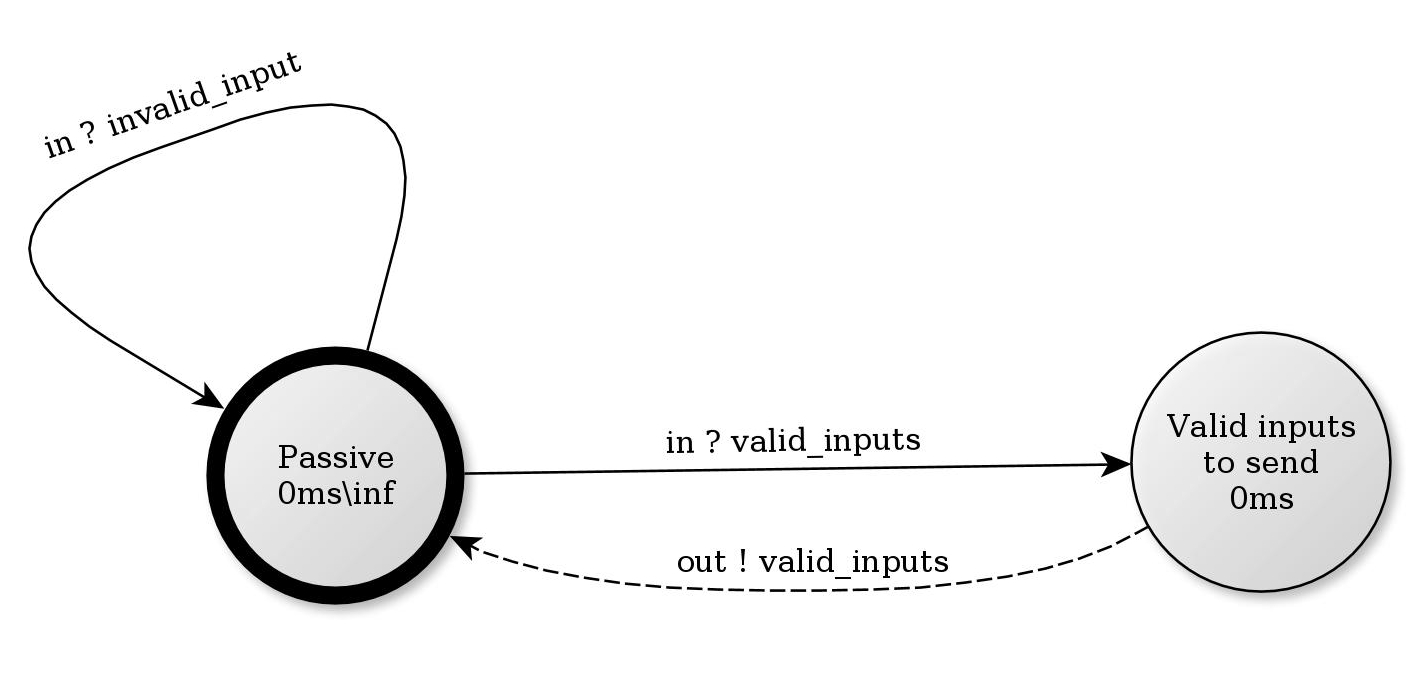
\includegraphics[width=1\textwidth]{atomic-filter.jpg}
 \caption{Filter atomic model.}
\end{figure}

\newpage
\subsection*{the enzyme}
The coupled model for an enzyme is the next:

\begin{figure}[h!]
 \centering
  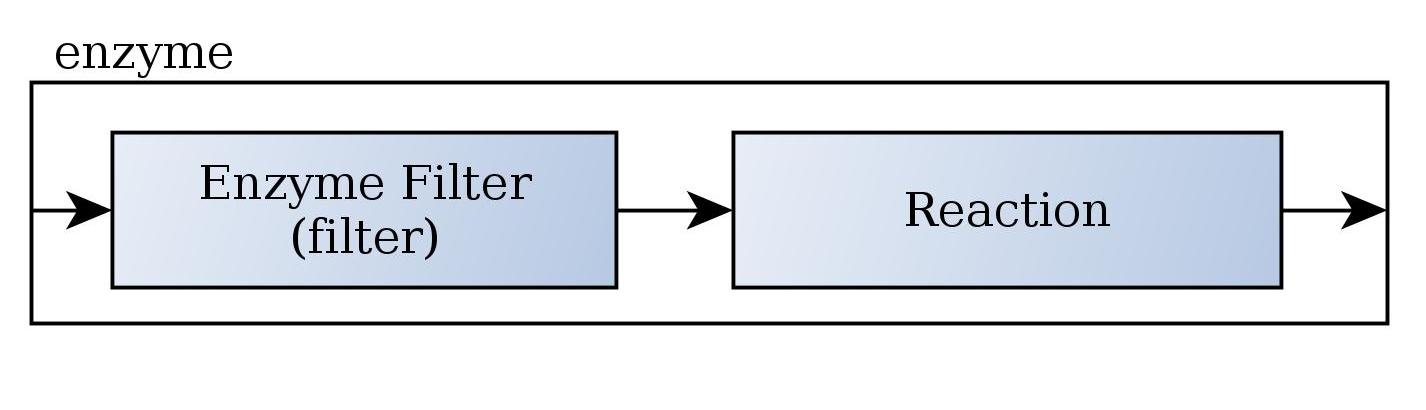
\includegraphics[width=1\textwidth]{coupled-enzyme.jpg}
 \caption{enzyme coupled model. blue color mean atomic models}
\end{figure}

\newpage

The reaction model, is who is in charge to bind the reactants/substrates and when all necessaries substrates are in the enzyme, the reaction start.
In every discrete interval of time (constant intervals), the reaction can lose one or more substrates that was bound to the enzyme, a random function with the appropriate distribution can decide in every interval of time which substrate will stay longer and which not.If a reaction is reversible and there is both substrates and products bound to the enzyme, the reaction cannot start until one of them (substrates or products) is gone.

moreover an enzyme represent a single unit who can catalyze only one unit of reactants producing only one unit of products, two enzyme cannot be in the same space, but probably, two enzyme of a same kind are attracted to stay close each other.
The next FSM represent the behavior of a reaction atomic model.

\begin{figure}[h!]
 \centering
  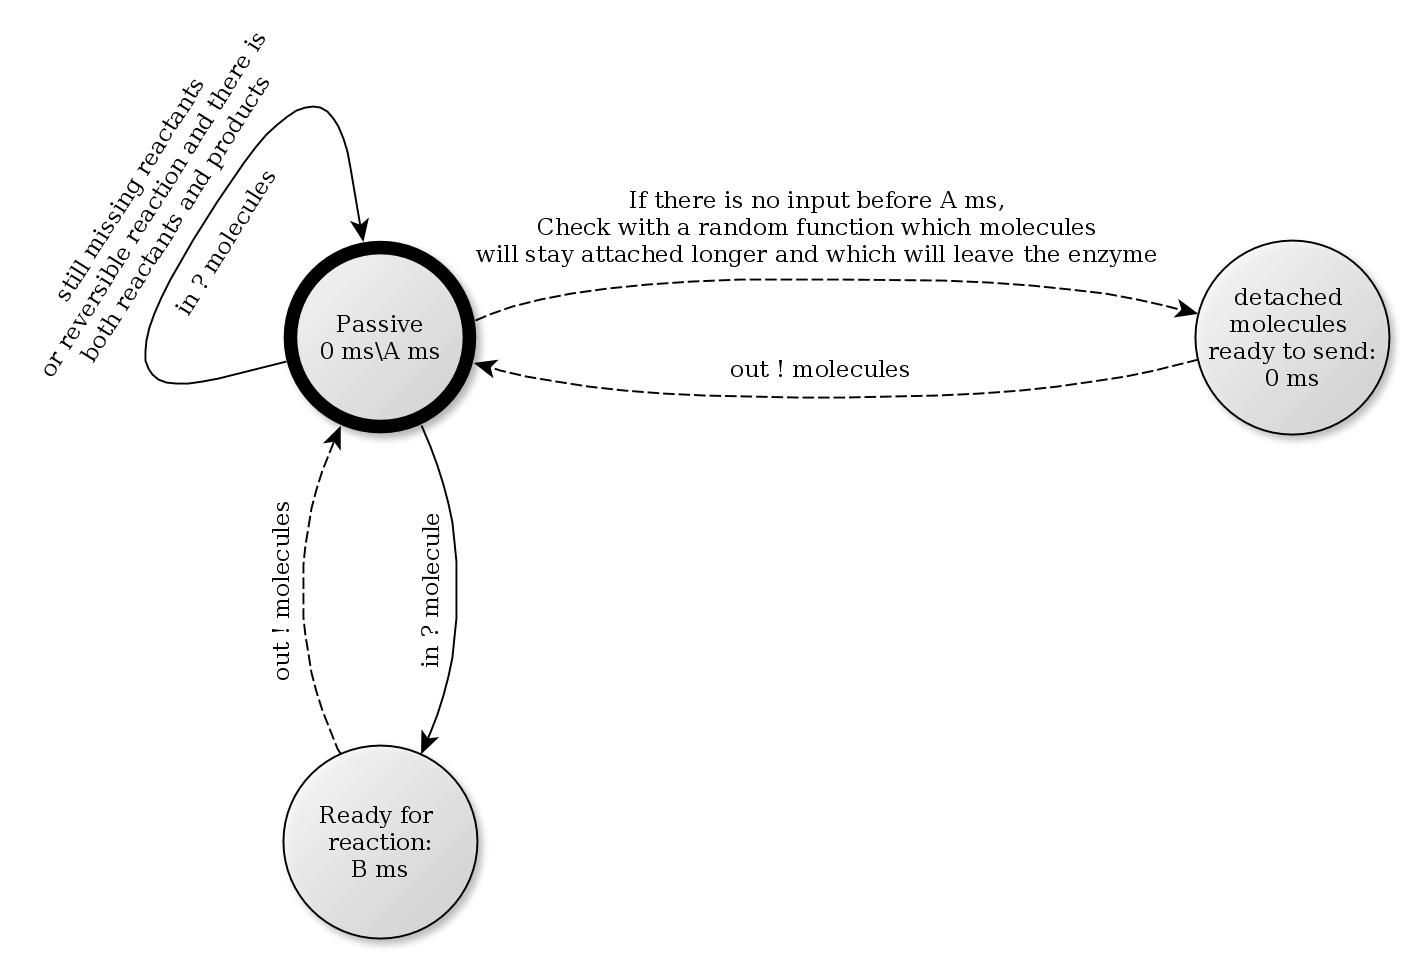
\includegraphics[width=1\textwidth]{atomic-reaction.jpg}
 \caption{Reaction atomic model.}
\end{figure}

\subsection*{the organelle}

The coupled model for an organelle is the next:

\begin{figure}[h!]
 \centering
  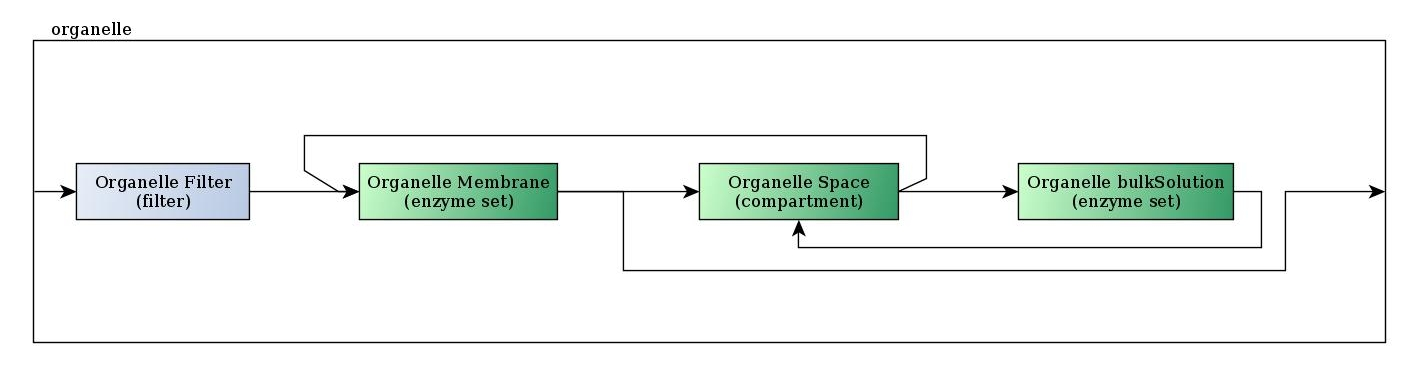
\includegraphics[width=1\textwidth]{coupled-organelle.jpg}
 \caption{organelle coupled model. blue color mean atomic models, green color mean coupled model}
\end{figure}

the coupled models Membrane, Compartment and Inner will be explained in the 3 next subsections. but just to understand the organelle model, here is a short explanation.

\subsubsection*{the Membrane}
this model has a list of enzyme and when a molecule arrive to the membrane if is bound to the correct enzyme, this enzyme start the transportation reaction and put the molecule in the output of the model to communicate the outside with the compartment model.

\subsubsection*{the compartment}
This model is basically a three dimensional space where the enzymes and molecules are moving and when a molecule is in the same place that an enzyme, the model will send the molecule to the enzyme model which correspond with this space.

\subsubsection*{Inner}
This mode is the same model that the Membrane model, the difference is that the enzyme located in the inner aren't transportation enzymes.

\subsubsection*{the organelle coupled model}
the molecules arrive to the membrane and after the transportation reaction happens it goes to the compartment where it will be moving until it found an enzyme and then, the compartment model send the molecule to the correct enzyme in the inner model, after the reaction occur, the inner model give back the output products to the compartment. Some times, moving molecule in the compartment can collapse with the edge of the tridimensional space and collapse with one enzyme in the membrane, in this case, the compartment send the molecule to the correct enzyme in the membrane and after the transportation reaction, the membrane will put the molecule in the output of the model.

\subsection*{the cytoplasm}
The coupled model for the cytoplasm is the next:

\begin{figure}[h!]
 \centering
  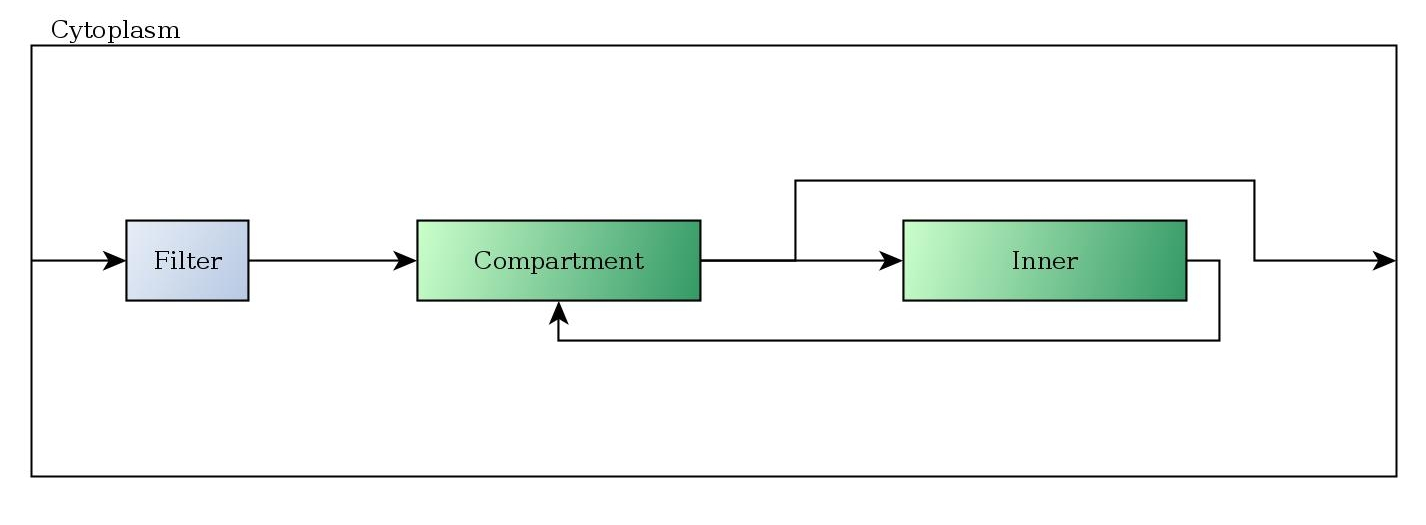
\includegraphics[width=1\textwidth]{coupled-cytoplasm.jpg}
 \caption{cytoplasm coupled model. blue color mean atomic models, green color mean coupled model}
\end{figure}

Is equal to an organelle model, with the main difference that the cytoplasm does not have membrane, the membrane who communicate the input molecule with the compartment of the cytoplasm is the cell membrane. So the compartment send the molecule to an external enzyme in the cell membrane or to an enzyme in an organelle membrane.

\subsection*{the compartment (space model)}

the coupled model for a compartment is the next:

\begin{figure}[h!]
 \centering
  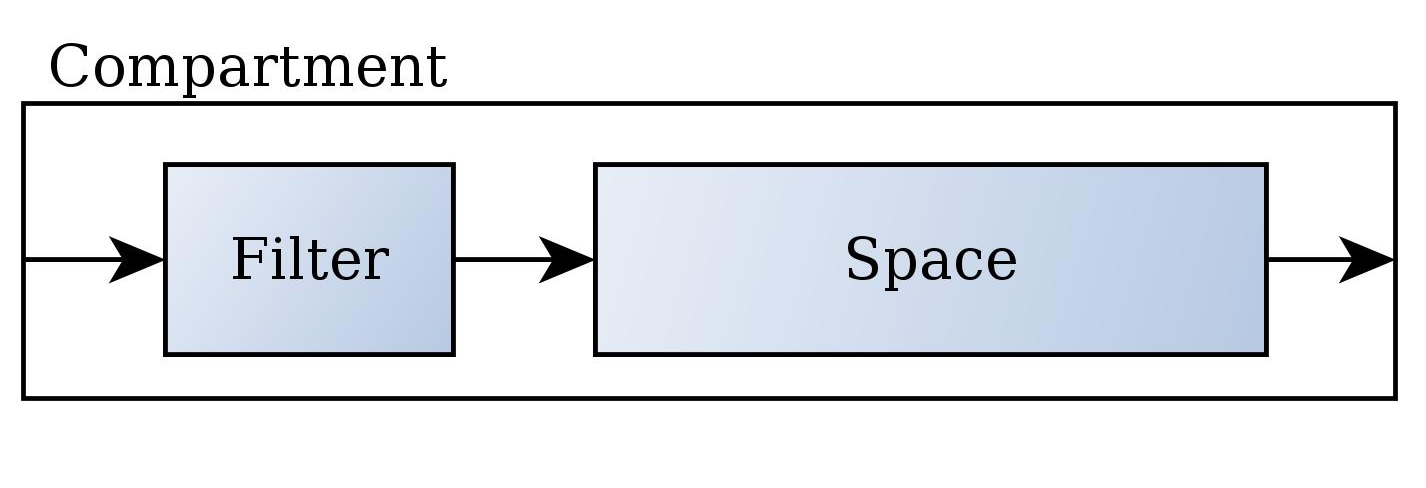
\includegraphics[width=1\textwidth]{coupled-compartment.jpg}
 \caption{compartment coupled model. blue color mean atomic models}
\end{figure}

The space is a model with a three dimensional set of discrete points, this set of point are the points that belongs to the compartment. each point have the information of the enzymes and/or molecules who are there. When a molecule is in the same space of a enzyme, the model will send this molecule to the remote model of the enzyme who take care of the reaction by the output in a message. 

The next FSM represent the behavior is a Space atomic model.


\begin{figure}[h!]
 \centering
  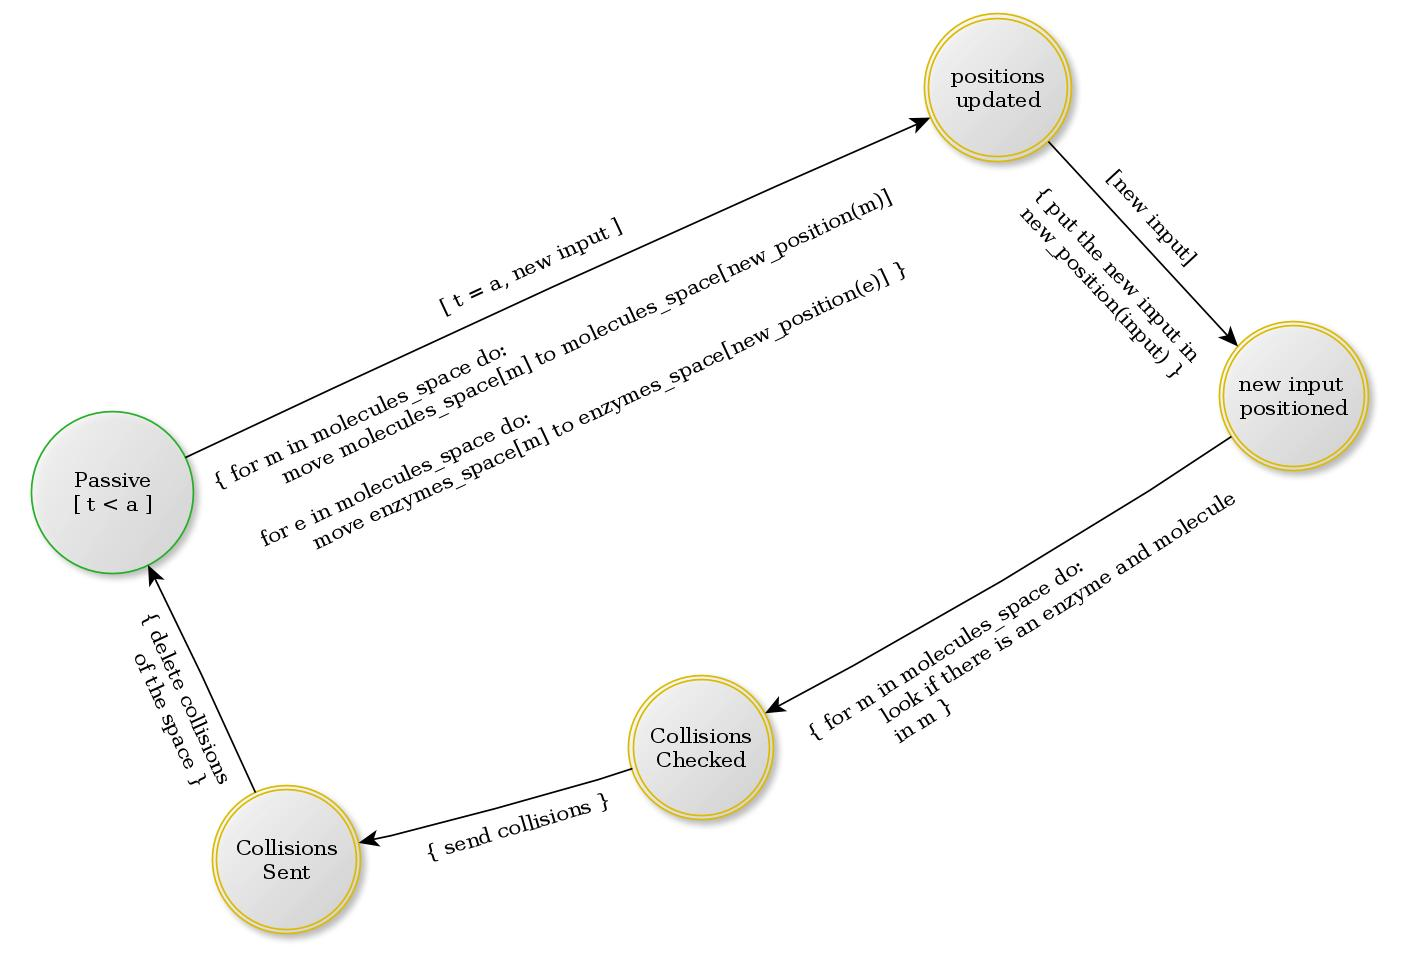
\includegraphics[width=320px]{atomic-space.jpg}
\end{figure}


\end{document}